\documentclass[varwidth,convert={density=500,outext=.png},border=0pt]{standalone}

% Tikz packages
\usepackage{tikz}
\usetikzlibrary{%
  patterns, plotmarks, backgrounds, shapes, arrows, calc, trees, positioning,
  chains, shapes.geometric, decorations.pathreplacing,
  decorations.pathmorphing, shapes.arrows, decorations.markings, quotes,
  arrows.meta, spy, fit, matrix
}

% General includegraphics and colour support
\usepackage{graphicx}
\usepackage{xcolor}
% Captions and subcaptions
\usepackage{caption}
\usepackage[labelformat=parens]{subcaption}

% String macros (for reading in tabular data)
\usepackage{xstring}

% PGFPlots
\usepackage{pgfplots}
\usepackage{pgfplotstable}
\pgfplotsset{compat=newest,plot coordinates/math parser=false}

%% Define node types
\tikzstyle{lnode} = [%
  circle,
  draw=black,
  minimum height=0.65cm,
  align=center,
  fill=none,
  text centered,
  inner sep=0.5pt,
  font=\tiny
]%

\begin{document}
  \begin{figure}
    \centering
    \scalebox{0.75}{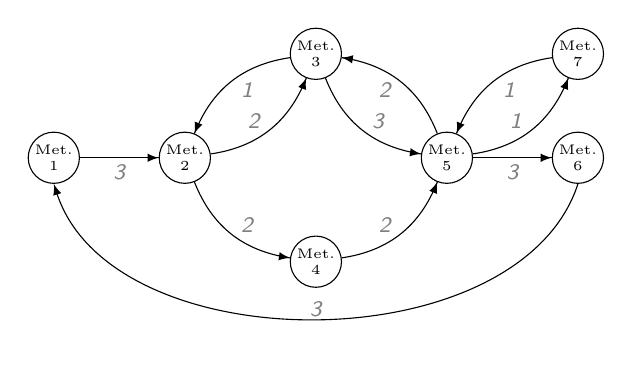
\begin{tikzpicture}[%
  >=latex,
  decoration={%
    markings,
    mark=at position 1.0 with {\arrow{>}}
  },
  every node/.style={%
    font=\sffamily\footnotesize\itshape,
    text=gray,
    text centered,
    align=center
  },
  frame/.style={draw=black,inner sep=2pt}
]

  % Nodes
  \node[lnode,text=black] (A1) {Met.\\1};
  \node[lnode,text=black,right=1.0cm of A1] (A2) {Met.\\2};
  \node[right=1.0cm of A2, lnode,text=black,yshift=1.32cm] (A3) {Met.\\3};
  \node[right=1.0cm of A2, lnode,text=black,yshift=-1.32cm] (A4) {Met.\\4};
  \node[right=1.0cm of A3, lnode,text=black,yshift=-1.32cm] (A5) {Met.\\5};
  \node[right=1.0cm of A5, lnode,text=black] (A6) {Met.\\6};
  \node[right=1.0cm of A5, yshift=1.32cm,lnode,text=black] (A7) {Met.\\7};

  % Intra-node edges
  \draw[postaction={decorate}] (A1) to node [below=0.1pt,yshift=1pt] {3} (A2);
  \draw[postaction={decorate}] (A2) to [bend right=30] node [above left=0.1pt,yshift=-3pt] {2} (A3);
  \draw[postaction={decorate}] (A3) to [bend right=30] node [below right=0.1pt,yshift=3pt] {1} (A2);
  \draw[postaction={decorate}] (A5) to [bend right=30] node [above left=0.1pt,yshift=-3pt] {1} (A7);
  \draw[postaction={decorate}] (A7) to [bend right=30] node [below right=0.1pt,yshift=3pt] {1} (A5);
  \draw[postaction={decorate}] (A3) to [bend right=30] node [above right=0.1pt,yshift=-3pt] {3} (A5);
  \draw[postaction={decorate}] (A5) to [bend right=30] node [below left=0.1pt,yshift=+3pt] {2} (A3);
  \draw[postaction={decorate}] (A2) to [bend right=30] node [above right=0.1pt,yshift=-3pt] {2} (A4);
  \draw[postaction={decorate}] (A4) to [bend right=30] node [above left=0.1pt,yshift=-3pt] {2} (A5);
  \draw[postaction={decorate}] (A5) to node [below=0.1pt,yshift=1pt] {3} (A6);

  % Boundary edges
  \draw[->,postaction={decorate}, bend left=72, distance=2.4cm] (A6.south) to node [above=0.1pt,yshift=-3pt] {3} (A1.south);

\end{tikzpicture}

}
    \vspace*{-1.18em}
  \end{figure}
\end{document}

